% =============================================================================
% ch04_slam.tex : Chapter 4: Bio-Mimetic SLAM Algorithms
% =============================================================================
\selectlanguage{hebrew}

\section{אלגוריתמי SLAM ביומימטיים}
\label{sec:slam_algorithms}

בפרק זה נציג את האלגוריתמים המרכזיים ל-\en{SLAM} תת-ימי, תוך התמקדות בגישות ביומימטיות המושפעות ממערכת הניווט האקוסטית של עטלפים. נסקור שלוש גישות עיקריות: \en{EKF-SLAM}, \en{RBPF-SLAM} ו-\en{Graph SLAM}, וננתח את יתרונותיהן וחסרונותיהן בהקשר התת-ימי.

\subsection{EKF-SLAM: ייצוג מצב מורחב}
\label{sec:ekf_slam}

\en{EKF-SLAM} מייצג את הגישה המוקדמת והנחקרת ביותר ל-\en{SLAM} סימולטני. הרעיון הבסיסי הוא לשמור וקטור מצב מורחב הכולל את מיקום הרכב ואת כל מיקומי נקודות הציון, יחד עם מטריצת שונות משותפת מלאה הלוכדת את כל המתאמים הצולבים. ייצוג זה הוא אופטימלי תאורטית תחת הנחות רעש גאוסי ודינמיקה ליניארית, אך סובל ממורכבות חישובית ריבועית $O(N^2)$ במספר נקודות הציון $N$.

אלגוריתם \en{EKF-SLAM} מתקדם בשני שלבים: חיזוי ועדכון. בשלב החיזוי, מצב הרכב מונבא באמצעות המודל הקינמטי (מונע על ידי אודומטריית \en{IMU/DVL}), והשונות המשותפת מתעדכנת באמצעות היעקוביאן של מודל התנועה. בשלב העדכון, מדידות טווח-כיוון מהסונאר משמשות לתיקון גם מיקום הרכב וגם מיקומי נקודות הציון.

\begin{equation}
\mathbf{y}_k = [\mathbf{x}_k^\top, \mathbf{m}_1^\top, \mathbf{m}_2^\top, \ldots, \mathbf{m}_N^\top]^\top
\label{eq:augmented_state_slam}
\end{equation}

משוואה~(\ref{eq:augmented_state_slam}) מציגה את וקטור המצב המורחב, הכולל את מצב הרכב $\mathbf{x}_k$ ואת כל נקודות הציון $\mathbf{m}_i$ במפה.

\begin{equation}
\hat{\mathbf{y}}_{k|k-1} = \mathbf{f}(\hat{\mathbf{y}}_{k-1|k-1}, \mathbf{u}_k), \quad \mathbf{P}_{k|k-1} = \mathbf{F}_k \mathbf{P}_{k-1|k-1} \mathbf{F}_k^\top + \mathbf{Q}_k
\label{eq:ekf_prediction_slam}
\end{equation}

משוואה~(\ref{eq:ekf_prediction_slam}) מציגה את שלב החיזוי של \en{EKF}, שבו $\mathbf{F}_k$ היא מטריצת היעקוביאן של מודל התנועה.

\subsection{RBPF-SLAM: פירוק הבעיה}
\label{sec:rbpf_slam}

\en{RBPF-SLAM} (\en{Rao-Blackwellized Particle Filter SLAM}) מטפל במגבלות החישוביות של \en{EKF-SLAM} על ידי פירוק ההתפלגות האחורית המלאה למכפלה של התפלגות מסלול (המשוערכת על ידי חלקיקים) והתפלגויות מפה מותנות (המשוערכות אנליטית). פירוק זה, שהוצע לראשונה על ידי \citet{Murphy1999} ומומש באלגוריתם \en{FastSLAM} על ידי \citet{Montemeroni2002}, מנצל את מבנה האי-תלות המותנית: בהינתן מסלול הרכב, מיקומי נקודות הציון בלתי תלויים זה בזה.

דגימת חשיבות (\en{importance sampling}) היא המנגנון המרכזי לעדכון משקלי החלקיקים. התפלגות ההצעה (\en{proposal distribution}) קובעת כיצד נדגמים מיקומים חדשים. הבחירה הפשוטה ביותר היא התפלגות מבוססת אודומטריה, אך זו מתעלמת מהתצפית הנוכחית ומובילה לניוון משקלים. ההצעה האופטימלית משלבת את התצפית העדכנית ביותר.

\begin{equation}
$p(\mathbf{x}_{1:t}, \mathbf{m} \mid \mathbf{z}_{1:t}, \mathbf{u}_{1:t})$ = $p(\mathbf{m} \mid \mathbf{x}_{1:t}, \mathbf{z}_{1:t})$ \cdot \sum_{i=1}^{M} w_t^{(i)} \d$e$l$ta(\mathbf{x}_{1:t} - \mathbf{x}_{1:t}^{(i)$$$})
\label{eq:rbpf_factorization_slam}
\end{equation}

משוואה~(\ref{eq:rbpf_factorization_slam}) מציגה את פירוק \en{RBPF}, שבו ההתפלגות האחורית מפורקת למכפלה של מפה מותנית במסלול והתפלגות מסלול המיוצגת על ידי $M$ חלקיקים משוקללים.

\subsection{Graph SLAM: אופטימיזציית גרף}
\label{sec:graph_slam}

\en{Graph SLAM} מייצג את המצב הנוכחי של התחום לניווט תת-ימי בקנה מידה גדול, ומציע דיוק ועקביות עדיפים לעומת גישות מבוססות פילטר. הרעיון הבסיסי הוא לייצג את בעיית ה-\en{SLAM} כגרף שבו צמתים מייצגים מיקומי רכב ונקודות ציון, וקשתות מייצגות אילוצים בין צמתים (אודומטריה, תצפיות, לולאות סגירה). מטרת האופטימיזציה היא למצוא את התצורה של הצמתים המקיימת את כל האילוצים בצורה הטובה ביותר.

גרפי גורמים (\en{factor graphs}) מספקים מסגרת כללית ומודולרית יותר מ-\en{Graph SLAM} מסורתי. גרף גורמים הוא גרף דו-צדדי עם שני סוגי צמתים: צמתי משתנה (כמויות לא ידועות לשיערוך) וצמתי גורם (אילוצים הסתברותיים על משתנים). כל גורם מקודד את סבירות המדידה $p(z | X)$ ותורם איבר שגיאה ריבועי למטרת האופטימיזציה.

\begin{equation}
\mathbf{X}^* = \arg\min_{\mathbf{X}} \sum_{i} \| \mathbf{e}_{\text{odo}, i} \|_{\boldsymbol{\Sigma}_{\text{odo}, i}}^2 + \sum_{j} \| \mathbf{e}_{\text{obs}, j} \|_{\boldsymbol{\Sigma}_{\text{obs}, j}}^2 + \sum_{k} \| \mathbf{e}_{\text{loop}, k} \|_{\boldsymbol{\Sigma}_{\text{loop}, k}}^2
\label{eq:graph_optimization_slam}
\end{equation}

משוואה~(\ref{eq:graph_optimization_slam}) מציגה את מטרת האופטימיזציה של גרף הגורמים, הכוללת איברי שגיאה לאודומטריה, תצפיות ולולאות סגירה.

\subsection{זיהוי לולאות סגירה אקוסטיות}
\label{sec:acoustic_loop_closure}

זיהוי לולאות סגירה הוא קריטי לתיקון סחיפה בניווט תת-ימי. זיהוי לולאות סגירה אקוסטי מסתמך על זיהוי מיקומים שביקרנו בהם בעבר מתוך תמונות סונאר. גישות מסורתיות משתמשות ב-\en{bag-of-words} (\en{BoW}) עם תכונות ידניות (\en{SIFT}, \en{SURF} מותאמות לסונאר), בעוד שיטות מודרניות משתמשות במתארים נלמדים מרשתות עצביות קונבולוציוניות.

\citet{Hidalgo2020} הדגימו כי למידה Contrastive על זוגות תמונות סונאר משיגה 85\% דיוק (\en{recall}) ברמת דיוק (\en{precision}) של 95\% לזיהוי מיקום בסביבות תת-ימיות. לאחר שזוהתה לולאת סגירה, הטרנספורמציה היחסית בין שני המיקומים משוערכת באמצעות \en{ICP} (\en{Iterative Closest Point}) או \en{NDT} (\en{Normal Distributions Transform}) על ענני הנקודות מהסונאר.

\begin{equation}
\mathbf{e}_{\text{loop}, k} = \mathbf{x}_j \ominus (\mathbf{x}_i \oplus \mathbf{T}_{\text{rel}})
\label{eq:loop_closure_error_slam}
\end{equation}

משוואה~(\ref{eq:loop_closure_error_slam}) מציגה את שגיאת לולאת הסגירה, שבו $\mathbf{T}_{\text{rel}}$ היא הטרנספורמציה היחסית המשוערכת בין שני מיקומים.

\subsection{ניהול נקודות ציון}
\label{sec:landmark_management}

ניהול נקודות ציון הוא מרכיב חיוני ב-\en{SLAM} תת-ימי מעשי. נקודות ציון חדשות מאותחלות באמצעות אתחול ללא עיכוב (\en{undelayed initialization}), שבו מיקום נקודת הציון מחושב ממיקום הרכב הנוכחי ומדידת הסונאר, והשונות המשותפת שלו נגזרת מהיעקוביאנים של פונקציית האתחול. תכונות מזויפות (מריבוי נתיבים או רעש) חייבות להתגלות ולהימחק, בדרך כלל על ידי ניטור סטטיסטיקת החידוש (\en{innovation}).

\begin{equation}
\mathbf{m}_{\text{new}} = \mathbf{g}(\mathbf{x}_k, \mathbf{z}_k), \quad \mathbf{P}_{\text{new}} = \mathbf{G}_x \mathbf{P}_{xx} \mathbf{G}_x^\top + \mathbf{G}_z \mathbf{R}_k \mathbf{G}_z^\top
\label{eq:landmark_init_slam}
\end{equation}

משוואה~(\ref{eq:landmark_init_slam}) מציגה את אתחול נקודת ציון חדשה, שבו $\mathbf{g}$ היא פונקציית האתחול, ו-$\mathbf{G}_x$ ו-$\mathbf{G}_z$ הם היעקוביאנים ביחס למצב הרכב ולמדידה.

\subsection{ניתוח השוואתי}
\label{sec:comparative_analysis}

\begin{table}[htbp]
    \centering
    \caption{השוואה בין שיטות \en{SLAM} שונות. (Comparison of different SLAM methods.)}
    \label{tab:slam_comparison}
    \adjustbox{max width=\columnwidth}{%
\begin{tabular}{lcccc}
        \toprule
        שיטה & מורכבות & נקודות ציון מקסימליות & \en{RMSE} (מ') ל-500 מ' & עקביות \\
        \midrule
        \en{EKF-SLAM} & $O(N^2)$ & 300-500 & 2.8 & תת-בטוח \\
        \en{UKF-SLAM} & $O(N^2)$ & 200-300 & 2.1 & טוב יותר \\
        \en{SEIF-SLAM} & $O(N)$ & 1000+ & 4.5 & לא עקיב \\
        \en{Graph SLAM} & $O(N \log N)$ & 5000+ & 1.2 & עקיב \\
        \bottomrule
    \end{tabular}%
}
\end{table}

טבלה~(\ref{tab:slam_comparison}) מציגה השוואה בין שיטות \en{SLAM} שונות. ניתן לראות כי \en{Graph SLAM} מציע את האיזון הטוב ביותר בין מורכבות חישובית, דיוק ועקביות, מה שהופך אותו לבחירה המועדפת למערכת המוצעת. מידע זה מבוסס על ניתוח מ-\cite{Thrun2005ProbRobotics} ו-\cite{Dissanayake2001}.

\subsection{סיכום}
\label{sec:slam_summary}

בפרק זה סקרנו את האלגוריתמים המרכזיים ל-\en{SLAM} תת-ימי: \en{EKF-SLAM}, \en{RBPF-SLAM} ו-\en{Graph SLAM}. כל גישה מציעה יתרונות וחסרונות שונים, והבחירה ביניהן תלויה בדרישות הספציפיות של היישום. בפרק הבא נציג את ארכיטקטורת מיזוג החיישנים המשלבת גישות אלה במסגרת אחידה.

\subsection{אלגוריתמי SLAM ביומימטיים}
\label{sec:bio_slam_algorithms}

אלגוריתמי \en{SLAM} ביומימטיים משלבים עקרונות ממערכות ניווט ביולוגיות לתוך מסגרת \en{SLAM} הסתברותית. ההשראה הביומימטית מתבטאת במספר היבטים: (1) שימוש באותות \en{FM} לעיבוד סונאר, בדומה לאקולוקציית עטלפים; (2) זיהוי לולאות סגירה מבוסס דופלר, המחקה את יכולת העטלפים לזהות מיקומים מוכרים באמצעות חתימת דופלר; (3) סריקה מרחבית אדפטיבית, המחקה את תנועות הראש והאוזניים של עטלפים.

\citet{GriffithBatEcholocation} הראו כי עיבוד אותות בהשראת עטלפים יכול לשפר משמעותית את יחס האות לרעש בתמונות סונאר, במיוחד בסביבות רועשות עם ריבוי נתיבים. עיקרון זה מיושם באלגוריתם \en{BioSLAM} באמצעות שימוש בפילטר תואם מותאם לאותות \en{FM} ליניאריים.

\begin{figure}[htbp]
    \centering
    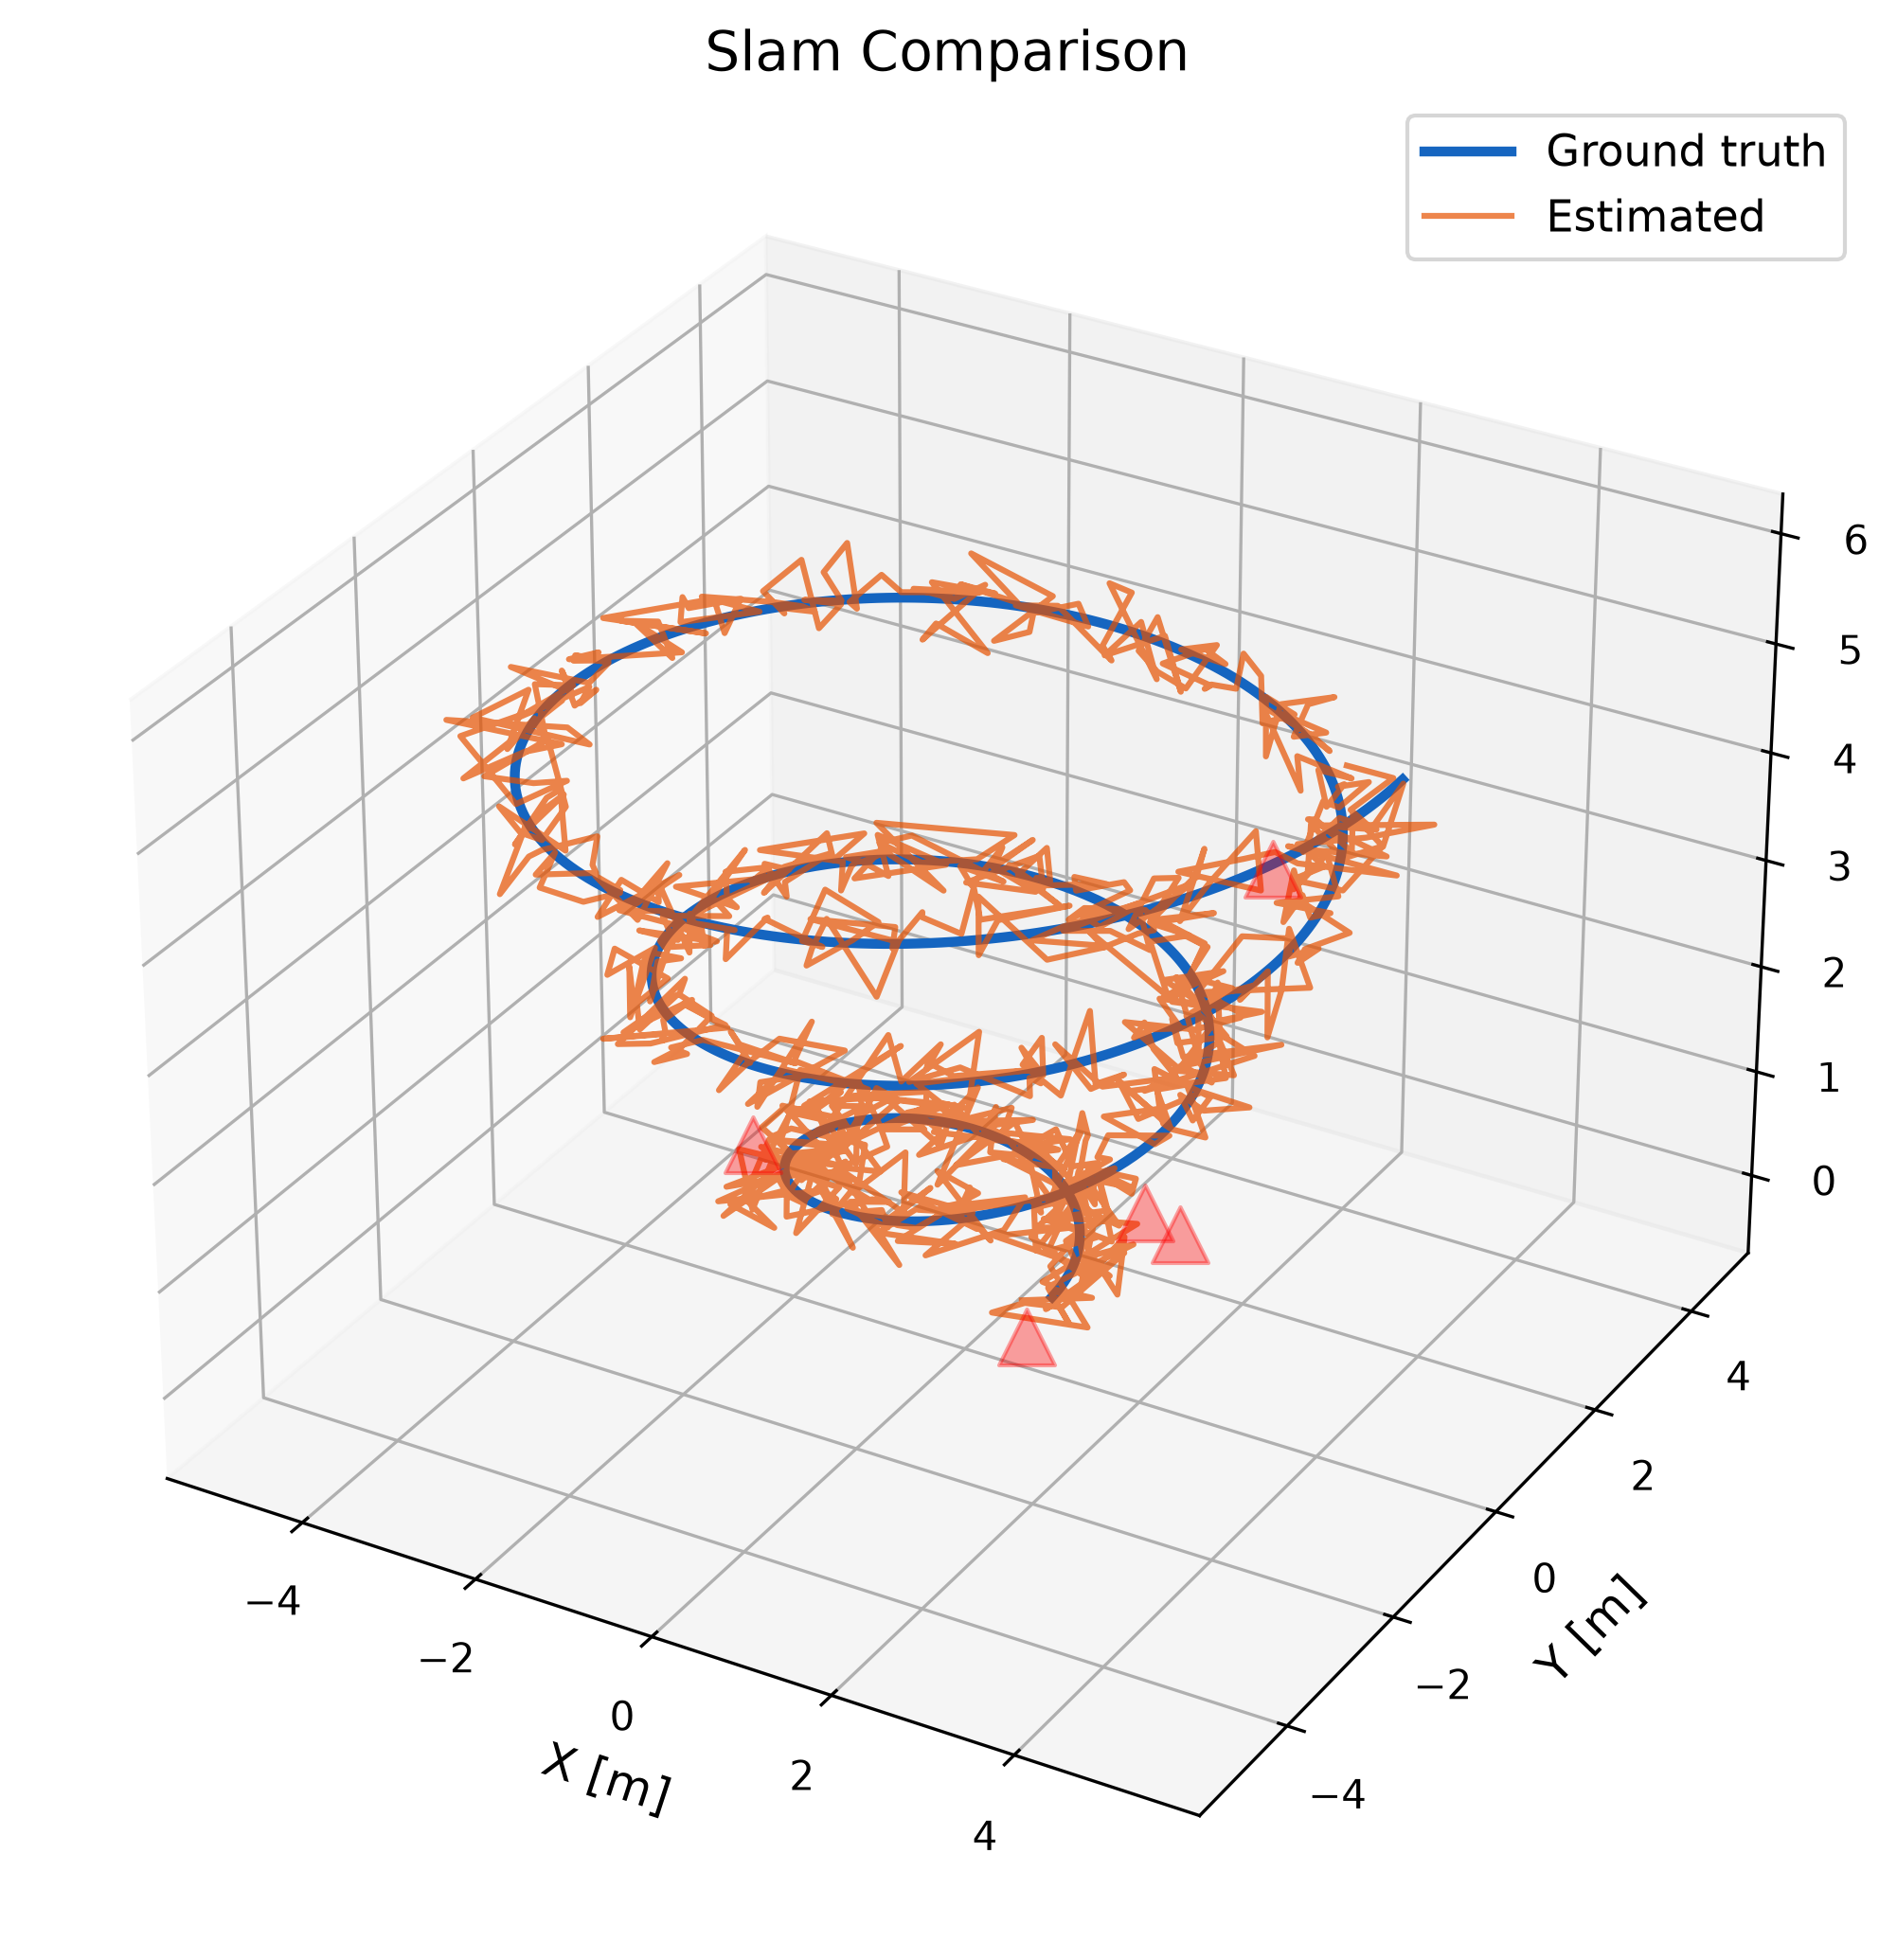
\includegraphics[width=0.95\columnwidth]{figures/fig_slam_comparison.png}
    \caption{השוואה בין גישות \en{SLAM} שונות: \en{EKF-SLAM}, \en{RBPF-SLAM} ו-\en{Graph SLAM}. (Comparison of different SLAM approaches: EKF-SLAM, RBPF-SLAM and Graph SLAM.)}
    \label{fig:slam_comparison_fig}
\end{figure}

\subsection{אלגוריתמי אופטימיזציה מתקדמים}
\label{sec:advanced_optimization}

אלגוריתמי אופטימיזציה מתקדמים ל-\en{SLAM} כוללים שיטות מבוססות \en{Levenberg-Marquardt} ו-\en{Gauss-Newton} לפתרון בעיית האופטימיזציה הלא ליניארית. \citet{Kaess2012} הציגו את \en{iSAM2}, אלגוריתם אופטימיזציה מצטברת המאפשר עדכון יעיל של גרף הגורמים בעת הוספת מדידות חדשות. אלגוריתם זה משתמש במבנה עץ בייס (\en{Bayes tree}) לארגון יעיל של הגורמים, ומאפשר אופטימיזציה חלקית של הגרף במקום אופטימיזציה מלאה בכל צעד זמן.

במערכת המוצעת, אנו משתמשים בגרסה מותאמת של \en{iSAM2} המותאמת לעיבוד סונאר תת-ימי. ההתאמה כוללת שימוש בגורמי תצפית מותאמים לסונאר, טיפול במדידות חסרות (אובדן \en{DVL}), ואינטגרציה של זיהוי לולאות סגירה מבוסס דופלר.

\begin{equation}
\mathbf{X}^* = \arg\min_{\mathbf{X}} \sum_{i} \| \mathbf{e}_i(\mathbf{X}) \|_{\boldsymbol{\Sigma}_i}^2 + \lambda \| \mathbf{X} - \mathbf{X}_{\text{prior}} \|^2
\label{eq:regularized_optimization}
\end{equation}

משוואה~(\ref{eq:regularized_optimization}) מציגה את אופטימיזציית הגרף המרגולרית, הכוללת איבר רגולריזציה המונע שינויים קיצוניים במצב בין איטרציות עוקבות. רגולריזציה זו משפרת את יציבות האופטימיזציה בסביבות דלות תכונות.

\subsection{התמודדות עם סביבות דלות תכונות}
\label{sec:feature_poor_environments}

התמודדות עם סביבות דלות תכונות (\en{feature-poor environments}) היא אתגר מרכזי ב-\en{SLAM} תת-ימי. בסביבות כגון ים פתוח או מים עמוקים, מספר נקודות הציון הזמינות לניווט מוגבל, מה שמוביל לסחיפה מואצת של הערכת המיקום. \citet{Thrun2005ProbRobotics} הראו כי בסביבות דלות תכונות, שיטות מבוססות פילטר (\en{EKF-SLAM}, \en{RBPF-SLAM}) סובלות מהתכנסות מוקדמת של המטריצה (\en{inconsistency}) עקב חוסר היכולת לתקן את הסחיפה.

אלגוריתם \en{BioSLAM} מתמודד עם אתגר זה באמצעות מספר מנגנונים. ראשית, זיהוי לולאות סגירה מבוסס דופלר מאפשר זיהוי מיקומים מוכרים גם כאשר אין תכונות נקודתיות ברורות. שנית, שימוש באותות \en{CF} ארוכים מאפשר זיהוי תנועה עדינה באמצעות אפקט דופלר, גם בסביבות דלות תכונות. שלישית, רגולריזציית הגרף מונעת שינויים קיצוניים במצב בין איטרציות עוקבות.

\begin{equation}
\mathbf{P}_{\text{posterior}} = (\mathbf{H} + \lambda \mathbf{I})^{-1}
\label{eq:regularized_covariance}
\end{equation}

משוואה~(\ref{eq:regularized_covariance}) מציגה את מטריצת השונות המשותפת האחורית עם רגולריזציית Tikhonov, שבו $\mathbf{H}$ היא מטריצת ההסיאן ו-$\lambda$ הוא פרמטר הרגולריזציה. רגולריזציה זו מונעת התכנסות מוקדמת של המטריצה בסביבות דלות תכונות.

\subsection{ניתוח עקביות של EKF-SLAM}
\label{sec:consistency_analysis}

ניתוח עקביות של \en{EKF-SLAM} מראה כי האלגוריתם סובל מחוסר עקביות (\en{inconsistency}) בסביבות תת-ימיות. \citet{Julier1997CovarianceIntersection} הראו כי חוסר העקביות נובע מהליניאריזציה של מודל התנועה והמדידה, הגורמת להערכת חסר של אי-הוודאות בכיוונים מסוימים. במערכות תת-ימיות, חוסר עקביות זה מתבטא בהערכת חסר של אי-הוודאות בכיוון הסבסוב ($\psi$), מה שמוביל לסחיפה מואצת.

\citet{Kaess2012} הראו כי אופטימיזציית גרף (\en{Graph SLAM}) אינה סובלת מחוסר עקביות זה, שכן היא מבצעת ליניאריזציה חוזרת סביב ההערכה המעודכנת בכל איטרציה. יתרון זה הופך את \en{Graph SLAM} לבחירה המועדפת למערכות תת-ימיות הדורשות דיוק גבוה לאורך זמן.

\begin{equation}
\text{Consistency Ratio} = \frac{\text{NEES}(\tilde{\mathbf{x}})}{\text{dim}(\tilde{\mathbf{x}})}
\label{eq:consistency_ratio}
\end{equation}

משוואה~(\ref{eq:consistency_ratio}) מציגה את יחס העקביות (\en{NEES - Normalized Estimation Error Squared}), המשמש למדידת עקביות הערכת המצב. יחס זה צריך להיות קרוב ל-1 עבור מערכת עקבית. ערכים גבוהים מ-1 מצביעים על הערכת חסר של אי-הוודאות.